\chapter{The Prediction}
% Covers: outline G4: the grid, 128 and 48 -- the coda. This chapter BORROWS NOTHING
% (that is its point). Chapter language (per Ch1's arrow plan): Geometry -- the grid
% drawn (the book's last figure).

\section{The door}
% Node-map: G4 whole, with the RECORD'S OWN PROVENANCE (turn 533): the 128 cells /
% 48 rungs are apparatus SETTINGS in the force route (the spring-scale re-pin of the
% gravity reading, matching the balance -- an internal cross-check); the record
% FENCES the 128 itself (not device-derived; "the reading FOR this grid seeding");
% the precedent: the alpha-route's own grid-128 seed is GONE (the crossing computed
% from device constants, no seed). THE PREDICTION, falsifiable: the two remaining
% seeds are EARNABLE and the derivation lands on 128 and 48 -- or fails in public.
% Door-not-wall; borrows nothing; THE FIGURE: the grid drawn.
% Gate: turn 533 (Ch9, ~1.5k budget). RIDER applied to Ch5 S1 (the interpolation
% framing -- marks assert, the reader interpolates).

An argument that claims to be an experiment owes the reader one thing more than its
results, its defenses, and its fences: it owes its next falsifiable claim. A
retrospective ends at a wall --- everything shown, everything settled, nothing at
stake ever again. An experiment ends at a door. This book has called itself an
experiment from its first page, and the fence chapter's closing sentence stated the
fee for that name: an argument that knows precisely where it stops has earned the
right to say what it expects next, and to be held to it. This chapter pays the fee.

It begins with a confession the reader is owed, though by now it will not surprise.
The book has never hidden an import, and two remain. Alongside the balance of
Chapter 5, the apparatus carries a second, independent route to the same gravity
reading --- a spring-scale route, re-pinning the balance's number by a different
mechanism, and matching it exactly: an internal cross-check, two instruments
agreeing on one value. That route's standard run is configured by two numbers: a
grid of one hundred twenty-eight cells, and forty-eight rungs of bisection. And
here the record's own honesty must be quoted, because the record fences these
numbers itself: the 128 is not device-derived --- no construction of the ground
earns it --- and the route's bracket is honestly stated in the record as the
reading for this grid seeding. Seeds, acknowledged as seeds, marked as such in
the apparatus: the last two numbers in this entire apparatus that were chosen
rather than earned. And the distinction deserves its own sentence rather than an
inference: the argument asserts only earned numbers --- Chapter 1 stands as
written --- while the apparatus carries, fenced and marked, these two seeds of a
route whose reading the record itself brackets as the reading for this seeding.
The book's claims are seedless; its workshop is not, yet, and says so.

Now the precedent, because the prediction stands on it. The flagship route once
carried exactly this kind of seed --- its own grid of one hundred twenty-eight,
imported to give the walk a lattice to work on. It is gone. The reader watched
the machinery that removed it: the crossing is computed from the device's own
constants --- the measured eighteen, its floor-plus-one five, the earned square
root --- no grid, no seed, no external number anywhere in the chain. The walk
earned away its seed, and the $\alpha$-route now runs seedless from ground to bracket.
What was done once, on the argument's most important route, is the pattern for
what the argument now predicts about its last two imports.

Here is the prediction, stated so it can fail. The two remaining seeds are
earnable: there exists a derivation, from the device's own constants and by the
device's own disciplines, of the force route's grid size and rung count --- the
same kind of derivation that freed the flagship route --- and when that
derivation is built and run cold, it lands on one hundred twenty-eight and
forty-eight. Not near them: on them, exactly, in the manner of every earned
number in this book. If it lands, the last imports retire, and the apparatus
becomes what the argument has been building toward: self-seeded end to end,
every number a receipt. If it lands elsewhere --- a derivation built in good
faith by this book's own rules, arriving at other values --- then the
prediction has failed in public, the fence around the seeds stands as the
record wrote it, and the reader will know the argument's reach ended here. Both
outcomes are stated in advance; only one of them was promised. That is what a
prediction is.

\begin{figure}[htbp]
\centering
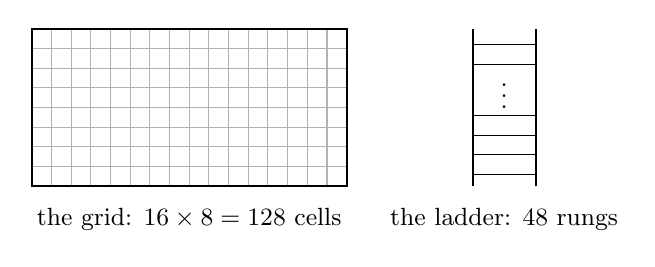
\begin{tikzpicture}[scale=1.0, every node/.style={font=\small}]
\draw[step=0.25, gray!60, thin] (0,0) grid (4,2);
\draw[thick] (0,0) rectangle (4,2);
\node[below] at (2,-0.15) {the grid: $16 \times 8 = 128$ cells};
\draw[thick] (5.6,0) -- (5.6,2);
\draw[thick] (6.4,0) -- (6.4,2);
\foreach \y in {0.15,0.4,0.65,0.9} \draw (5.6,\y) -- (6.4,\y);
\node at (6.0,1.25) {$\vdots$};
\foreach \y in {1.55,1.8} \draw (5.6,\y) -- (6.4,\y);
\node[below] at (6.0,-0.15) {the ladder: $48$ rungs};
\end{tikzpicture}
\caption{The last two seeds, drawn: the force route's grid of one hundred
twenty-eight cells and its ladder of forty-eight bisection rungs. The prediction
is that this picture is derivable --- that a construction from the device's own
constants, built by this book's rules and run cold, arrives at exactly these two
numbers, the way the flagship route's walk earned away its own seed. If it
arrives anywhere else, the prediction has failed, in public, here.}
\end{figure}

The reader will notice that this chapter cites no one and borrows nothing --- no
ledger row lands here, and that is its point, stated plainly as the map promised.
A prediction is the one genre in which borrowed authority is worth nothing at
all: no tradition can make the derivation land on one hundred twenty-eight, and
no great name can excuse it if it lands elsewhere. The chapter stands on the
argument behind it or it does not stand.

And so the book ends the way an experiment ends: mid-motion, with its next
measurement named and its neck extended. The claim was stated whole in the first
chapter and earned across seven more; the readings were made, defended, and
fenced; the ring was proved closed; the falsifiers stand gathered in their
table, one already fired and survived. The book was arranged to survive the
reader who attacks it. It is arranged, now, to be survived or killed by the
measurement it names --- and it prefers that arrangement to any safer ending,
because the alternative was to be a retrospective, and the first page promised
an experiment. The ring is closed. The door is open.
